
%% bare_conf.tex
%% V1.4a
%% 2014/09/17
%% by Michael Shell
%% See:
%% this can cause conflict
%% http://www.michaelshell.org/
%% for current contact information.
%%
%% This is a skeleton file demonstrating the use of IEEEtran.cls
%% (requires IEEEtran.cls version 1.8a or later) with an IEEE
%% conference paper.
%%
%% Support sites:
%% http://www.michaelshell.org/tex/ieeetran/
%% http://www.ctan.org/tex-archive/macros/latex/contrib/IEEEtran/
%% and
%% http://www.ieee.org/

%%*************************************************************************
%% Legal Notice:
%% This code is offered as-is without any warranty either expressed or
%% implied; without even the implied warranty of MERCHANTABILITY or
%% FITNESS FOR A PARTICULAR PURPOSE! 
%% User assumes all risk.
%% In no event shall IEEE or any contributor to this code be liable for
%% any damages or losses, including, but not limited to, incidental,
%% consequential, or any other damages, resulting from the use or misuse
%% of any information contained here.
%%
%% All comments are the opinions of their respective authors and are not
%% necessarily endorsed by the IEEE.
%%
%% This work is distributed under the LaTeX Project Public License (LPPL)
%% ( http://www.latex-project.org/ ) version 1.3, and may be freely used,
%% distributed and modified. A copy of the LPPL, version 1.3, is included
%% in the base LaTeX documentation of all distributions of LaTeX released
%% 2003/12/01 or later.
%% Retain all contribution notices and credits.
%% ** Modified files should be clearly indicated as such, including  **
%% ** renaming them and changing author support contact information. **
%%
%% File list of work: IEEEtran.cls, IEEEtran_HOWTO.pdf, bare_adv.tex,
%%                    bare_conf.tex, bare_jrnl.tex, bare_conf_compsoc.tex,
%%                    bare_jrnl_compsoc.tex, bare_jrnl_transmag.tex
%%*************************************************************************

\documentclass[conference]{IEEEtran}

% graphicx is a very useful package for inserting graphics into your paper. See
% below for more information and examples
\ifCLASSINFOpdf
\usepackage[pdftex]{graphicx}
  % declare the path(s) where your graphic files are
  % \graphicspath{{../pdf/}{../jpeg/}}
  % and their extensions so you won't have to specify these with
  % every instance of \includegraphics
  % \DeclareGraphicsExtensions{.pdf,.jpeg,.png}
\else
  % or other class option (dvipsone, dvipdf, if not using dvips). graphicx
  % will default to the driver specified in the system graphics.cfg if no
  % driver is specified.
  % \usepackage[dvips]{graphicx}
  % declare the path(s) where your graphic files are
  % \graphicspath{{../eps/}}
  % and their extensions so you won't have to specify these with
  % every instance of \includegraphics
  % \DeclareGraphicsExtensions{.eps}
\fi
% graphicx was written by David Carlisle and Sebastian Rahtz. It is
% required if you want graphics, photos, etc. graphicx.sty is already
% installed on most LaTeX systems. The latest version and documentation
% can be obtained at: 
% http://www.ctan.org/tex-archive/macros/latex/required/graphics/
% Another good source of documentation is "Using Imported Graphics in
% LaTeX2e" by Keith Reckdahl which can be found at:
% http://www.ctan.org/tex-archive/info/epslatex/
%
% latex, and pdflatex in dvi mode, support graphics in encapsulated
% postscript (.eps) format. pdflatex in pdf mode supports graphics
% in .pdf, .jpeg, .png and .mps (metapost) formats. Users should ensure
% that all non-photo figures use a vector format (.eps, .pdf, .mps) and
% not a bitmapped formats (.jpeg, .png). IEEE frowns on bitmapped formats
% which can result in "jaggedy"/blurry rendering of lines and letters as
% well as large increases in file sizes.
%
% You can find documentation about the pdfTeX application at:
% http://www.tug.org/applications/pdftex

\begin{document}

% paper title
\title{A Comparison of Search Algorithms\\ on the Tower of Hanoi Problem  }

% author names and affiliations
\author{\IEEEauthorblockN{Wen Chuan Lee}
\IEEEauthorblockA{College of Science and Engineering\\
University of Minnesota, Twin Cities\\
Minneapolis, MN\\
Email: lee@leewc.com - leex7095@umn.edu}
}
% make the title area
\maketitle

% As a general rule, do not put math, special symbols or citations
% in the abstract
\begin{abstract}
This paper compares the performance of 4 major search algorithms, the Breadth First Search, Bidirectional Breadth First Search, Depth First Search as well as Iterative Depth First Search on the Tower of Hanoi. The comparison is done empirically based on concrete experiments and metrics such as runtime as well as nodes traversed to find a solution. In the experiment, Depth first search is the fastest and most memory efficient algorithm in solving the Tower of Hanoi, whereas Bidirectional Breadth First Search is the second fastest. The Tower of Hanoi problem was selected as the problem to be researched as the puzzle has multiple states and rules to be followed, with large search spaces as the number of disks are added.

\end{abstract}

\section{Introduction}

\subsection{The Field of Search}
Since the late 1950s, search has been considered to be influential to the field of Artificial Intelligence. Early AI programs had an algorithm that would search through possible states to arrive at an eventual solution, some even being able to backtrack when the algorithm reached a dead end. This paradigm was considered by McCorduck and others to be "reasoning by search" \cite{McCorduck01}. Search has also been an important to the field of computer science as it allows information to be gathered from data in a manner that would be nowhere fast nor accurate enough if done by human beings. There has been much emphasis on this field as computers aim to simplify our increasingly information-oriented lives. A good search algorithm not only provides the right results, but also accurate, precise and as efficient and possible. With the great increase in computing power, search algorithms are even used to solve puzzles and derive logic based on a set of rules, this can be demonstrated with the Towers of Hanoi.

\subsection{The Tower of Hanoi Problem}

The Tower of Hanoi is a mathematical and logical toy problem that has exactly 3 pegs with a varying number of disks. The goal state of the problem is to have all disks moved from one peg to another peg with regards to specific rules.The complexity of the problem increases exponentially with the increased number of disks. This is because with \textit {n} number of disks, the \textit{minimum} number of moves required to solve the Towers of Hanoi puzzle is $2^{n} - 1$. \cite{FamousPuzzles}

This mathematical problem has 3 simple rules:

\begin{enumerate}
\item Only one disk can be moved at a time.
\item A larger disk cannot be moved on top of a smaller disk.
\item Only the top most disk of each peg can be moved to another peg. 
\end{enumerate}

In this paper I attempt to make an experimental analysis on the performance and memory of complexity of the 4 search algorithms on the Tower of Hanoi problem. The Tower of Hanoi problem was selected as the problem to be researched as the puzzle has multiple states and rules to be followed, with large search spaces as the number of disks are added. The problem will be represented in Python along with the search algorithms, after which problems of varying difficulty are provided to the algorithm by increasing the number of disks in the problem. Finally I will analyze and discuss the memory used and the time complexity of each algorithm to solve each of the problem, and provide some insight on the most performant algorithm based on time and memory that solves the Tower of Hanoi problem. The data collected will display a major difference of the runtime between algorithms to provide clarity on how the performance of these algorithms work. 

The paper is organized as follows, the next section discusses the algorithms on a theoretical level, in which complexity is discussed. This is followed by a discussion on the experimental set up, and then presentation of the raw data. An analysis and discussion based on the data is then provided, and finally a conclusion that explores possible further research.

\subsection{The Algorithms}

One of the more well-known algorithms of search is the breadth-first search (BFS). As an uninformed search algorithm, BFS expands the root node and then the successors of the root node, followed by their successors and so on \cite{Textbook01}. All nodes at a specific depth are searched before the following depth are expanded. An advantage of the BFS algorithm is that it is complete, in which breadth first search will eventually find a solution that exists in the state space, if the branching factor is finite. The solution found by BFS is also optimal if and only if the path cost is a nondecreasing function of the depth of the node \cite{Textbook01}.

Bidirectional breadth-first search (bidirectional BFS) is a modified version of BFS in which two simultaneous BFS searches are started, one from the initial state and one from the final state. However, the key difference is that instead of a goal state test at every level, this is replaced by a check to see if the two frontiers have an intersecting node. If there is one, then the solution path is found. The distinction on this is the assumption that the sum of 2 simultaneous searches will be less than the complexity of a single search from the initial state. 

Depth First Search (DFS) is another uninformed search algorithm that traverses down a tree vertically unlike the horizontal breadth first search. The algorithm will arrive at a solution faster if the path that is being traversed down is the solution path (i.e, contains the goal state). Upon finding an no other child nodes to traverse down to, the algorithm will then go back to the previous node and explore another node at the same level. There are 2 implementations of DFS, in which one is iterative, and the other recursive. This paper explores DFS using the iterative implementation.

Iterative Deepening Depth First Search (IDDFS) is a modification of DFS, but instead of traversing down the search tree until no possible child nodes are generated before backtracking, IDDFS has a maximum depth of traversal that increases by 1 and then restarting the search again at each iteration from the top. The algorithm terminates when a solution is found. By restarting the search and limiting the maximum depth, this would avoid the algorithm going endlessly going down the search tree and yield a solution state faster if the state is contained in the middle or the right side of the search tree. Despite being a depth first search, this depth limited search visits nodes in a breadth first fashion cumulatively. 


\section{Hypothesis and Theoretical Analysis}

The best algorithm in terms of performance and time complexity is Depth First Search. While Bidirectional BFS will have a better performance and runtime than BFS itself, DFS triumphs both algorithms in terms of finding a solution state for the Towers of Hanoi. Whereas BFS has to explore each node at every level before moving on to the next, the memory and time required will be much longer while Bidirectional BFS will reduce the time of exploring each node at every level by running two simultaneous searches, that is one originating from the problem state and one originating from the goal state. Finally, runtime of IDDFS will be in between the runtime of Bidirectional BFS and BFS  as the search will continuously restart. This property of this algorithm is believed to make IDDFS unsuitable for finding solutions that are always located in the leaves of a search tree.

Both BFS and bidirectional BFS are both complete and optimal if the step costs are all identical (in the case of the Towers of Hanoi problem they are). As bidirectional BFS uses BFS in both simultaneous searches, the algorithm shares the complete and optimal properties of BFS. IDDFS is also complete and optimal given the nature of the algorithm's traversal. DFS is not will not yeild an optimal solution and is not complete.  

The difference however, is the theoretical bounds on time and space. For BFS, the time and space complexity is 

\begin{equation}
 O(b^d)
\end{equation}

where \textit{b} is the branching factor of the tree and \textit{d} is the depth of the tree. Specifically for the Towers of Hanoi problem to be represented, the branching factor will be 1 or 2 as only the top most pegs can be moved at each time, and moving back to a previous state is considered useless and does not cause the algorithm to arrive closer to the goal state. Therefore, the depth of the tree for this solution will be:

\begin{equation}
d = 2^n - 1
\end{equation}

For Bidirectional BFS, the time and space complexity will be 

\begin{equation}
 O(b^{d/2})
\end{equation}

By having 2 simultaneous searches, bidirectional BFS attempts to run in less than the time and space complexity of BFS. If 
the following is true then bidirectional BFS will be much faster than running a single BFS algorithm only. \cite{Textbook01}

\begin{equation}
O(b^{d/2}) + O(b^{d/2}) \leq O(b^d)
\end{equation}

Depth First Search runs with 
\begin{equation}
 O(b^{d})
\end{equation}

for space and time complexity where d is the maximum depth limit traversed. Whereas Iterative Deepening Depth First Search (IDDFS) will have a time complexity of \begin{equation}
O(b^{d})
\end{equation} as well, but only a space complexity of \begin{equation} O(bd)\end{equation} as less memory is used for node storage on limited depths. Although the states are visited multiple times which may seem as a wasteful action, the behavior is not too costly as most of the nodes are at a lower level, making the multiple visits at the higher levels have less impact on performance.


\section{Experimental Set-Up}
The set up for testing both algorithms will be done by varying the number of disks, \textit{n}. This increases the size of the graph as well as the depth of the graph of states. A state graph (that also contains illegal actions) has a maximum of $3^n$ nodes for a 3-peg Tower of Hanoi problem. The solution depth will have a size of $2^n-1$ as previously mentioned.

The Tower of Hanoi problem is abstracted by representing each peg as a list, and the entire set up that consists of 3 pegs into another list, yield a state that is represented as a list of lists of integers. A sentinel value, which is a value to indicate the end of data (commonly used in searching \cite{CodeComplete}) is used to represent that no more disks are on a particular peg. The sentinel values have a value of {n+1} where {n} is the total number of disks this allows for simplified implementation and faster computations.

The initial state will be when all disks are on the first peg, and the goal state is when all disks are placed in order from largest to smallest on the third peg. Pruning was built into the problem framework by ensuring that possible states generated conformed to the rules in the Tower of Hanoi, ensuring that illegal states (larger disks on top of smaller disks, moving multiple disks at a time without a specific order) are not generated, to reduce the size of the search space and avoid unnecessary computation by generating and traversing down a branch of states that will not arrrive to a legal solution state. A dictionary of visited states are also kept in memory to ensure algorithms are not caught in a loop revisiting the same states infinitely. The key of the dictionary is a string representation of the state, and the value is either an integer of 1, or the actual reference to the node, this allows us to fetch the node for bidirectional BFS when a solution is found.

After running all 4 algorithms with an increasing number of disks and recording the number of nodes traversed to find a solution as well as the total computation time to find the solution, a graph of Number of Nodes Traversed to the Number of Disks will be generated, where both the algorithms can be compared. A graph of Computation time to the Number of Disks will also be generated for a concrete analysis of algorithms.

The experiments where then executed on a Intel® Core™ i7-4790 machine running at 3.60GHz with 32GB of RAM. The computer used was a lab computer that had SSH access as well as the ability to keep background processes executing with the screen utility. The experiment ran for over 30 hours taking up over 6 GB of RAM. The experiment was halted at 11 disks because of the exponential increase in runtime.

\section{Results}

\subsection{Maximum Size of Frontier by Number of Disks}

\begin{tabular}{ | p{0.97cm} | p{1cm} | p{2cm} | p{1cm} | p{1.2cm} |}
    \hline
    Number of \ Disks & Depth First \ Search & Bidirectional \ BFS & Breadth \ First Search & Iterative Deepening \ DFS \\ \hline
    2 & 4 & 3 & 3 & 5 \\ \hline
    3 & 9 & 8 & 14 & 10 \\ \hline
    4 & 28 & 21 & 36 & 29 \\ \hline
    5 & 81 & 79 & 156 & 82 \\ \hline
    6 & 244 & 254 & 528 & 245 \\ \hline
    7 & 729 & 1079 & 2164 & 730 \\ \hline
    8 & 2188 & 4247 & 8256 & 2189 \\ \hline
    9 & 6561 & 16599 & 33236 & 6562 \\ \hline
    10 & 19684 & 66135 & 131328 & 19685 \\ \hline
    11 & 59049 & 262999 & 526164 & 59050 \\ \hline
\end{tabular}

\begin{figure}
\centering
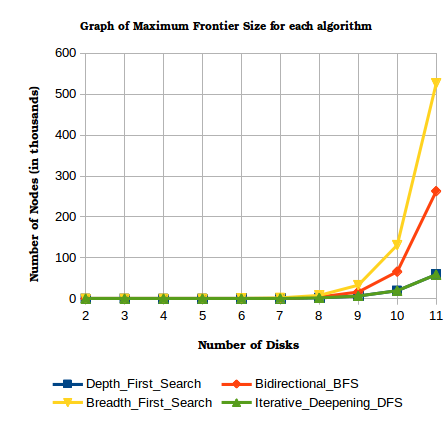
\includegraphics[width=3.7in]{hanoi_maxFrontier}
\caption{Graph of Maximum Frontier Size to Number of Disks }
\label{fig:my_label}
\end{figure}

\begin{table*}[t]
\subsection{Runtime (seconds) of each algorithm to Number of Disks}
\begin{tabular}{ |l |l |l |l |l |}
    \hline
    Number of \ Disks & Depth First \ Search & Bidirectional \ BFS & Breadth \ First Search & Iterative Deepening \ DFS \\ \hline
    2 & 0.000156392 & 0.000212669 & 0.000096286 & 0.000472911 \\ \hline
    3 & 0.000204044 & 0.000455272 & 0.000719421 & 0.000987642 \\ \hline
    4 & 0.000950633 & 0.001794590 & 0.003294816 & 0.009155311 \\ \hline
    5 & 0.002016366 & 0.007936978 & 0.017867410 & 0.055075039 \\ \hline
    6 & 0.006868233 & 0.041572044 & 0.106164721 & 0.537936986 \\ \hline
    7 & 0.012976039 & 0.265300220 & 0.740262595 & 4.933634893 \\ \hline
    8 & 0.067659920 & 2.026069019 & 6.571621341 & 55.26996347 \\ \hline
    9 & 0.128477633 & 16.297773958 & 52.6292188720 & 744.907908745 \\ \hline
    10 & 0.726265783 & 118.008149897 & 389.933532058 & 8319.07307241 \\ \hline
    11 & 1.543463721 & 900.394615177 & 3774.456782876 & 84143.691529322 \\ \hline
\end{tabular}
\end{table*}

\begin{figure}
\centering
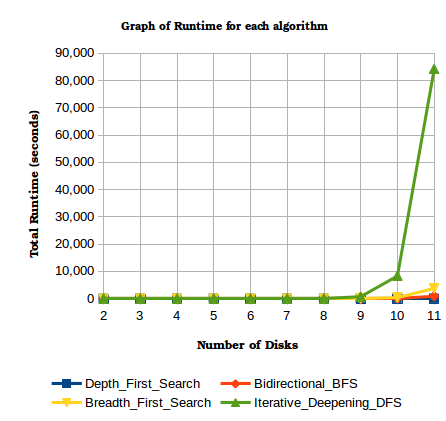
\includegraphics[width=3.7in]{hanoi_runtime}
\caption{Graph of Runtime (seconds) to Number of Disks }
\label{fig:my_label2}
\end{figure}

\subsection{Number of Nodes Traversed to Number of Disks}

\iffalse
\begin{tabular}{ | p{0.97cm} | p{1cm} | p{1.5cm} | p{2cm} | p{1.2cm} |}
    \hline
    Number of \ Disks & Depth First \ Search & Bidirectional \ BFS & Breadth \ First Search & Iterative Deepening \ DFS \\ \hline
2 & 6 & 10 & 5 & 28 \\ \hline
3 & 9 & 22 & 36 & 55 \\ \hline
4 & 49 & 86 & 184 & 534 \\ \hline
5 & 81 & 486 & 1194 & 3403 \\ \hline
6 & 428 & 2506 & 6738 & 30992 \\ \hline
7 & 729 & 15182 & 43288 & 266815 \\ \hline
8 & 3831 & 91516 & 257792 & 2404618 \\ \hline
9 & 6561 & 542326 & 1606086 & 21533203 \\ \hline
10 & 34450 & 3286532 & 9671326 & 193828356 \\ \hline
11 & 59049 & 19768542 & 59096340 & 1743480775 \\ \hline
\end{tabular}
\fi

\begin{figure}
\centering
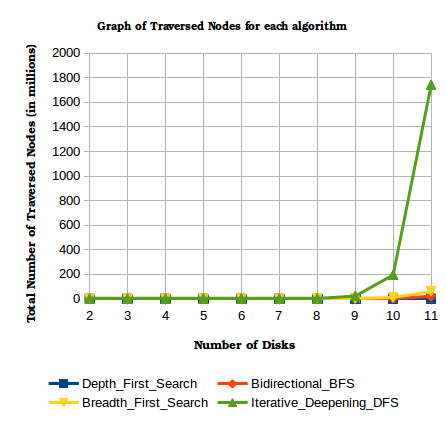
\includegraphics[width=3.5in]{hanoi_traversedNodes}
\caption{Graph of Number of Traversed Nodes to Number of Disks }
\label{fig:my_label3}
\end{figure}


\section{Results Discussion}
From the results it can be seen that Depth First Search is the fastest algorithm to obtain a goal state that is the solution. This is expected as the solutions are always deeper down the tree. Bidirectional Breadth First Search is the second fastest algorithm, although the algorithm takes an exponentially larger amount of time to solve larger number of disks. Although bidirectional BFS still yields a solution by over a factor of 2 faster than a single instance of the BFS. The results generated for number of nodes traversed, runtime and maximum size of frontier all confirm this. Bidirectional BFS manages to reduce the depth traversed by separating the problem into 2 instances (from initial state and goal state) as there are lesser number of nodes at shallow levels. This greatly reduces the number of states to visit before obtaining a solution. Iterative Deepening DFS however yielded the worst performance, as nodes are constantly revisited as the search is restarted, and the Tower of Hanoi problem only has solutions stored in the deepest level of the tree. This caused the algorithm to perform badly in terms of memory and runtime.

There are negligible differences between the algorithms on small number of disks, but as the Tower of Hanoi problem increases in complexity exponentially as the number of disks increases, the difference is evident. On a problem with 11 disks, DFS only took 1.54 seconds to find a solution, while Bidirectional BFS took 900.4 seconds (15 minutes), and BFS took 3774.5 seconds (1.04 hours), and Iterative Deepening DFS took 84143.70 seconds (23.4 hours) to find the solution. 

From the results, we are able to prove that the Iterative Deepening DFS algorithm do not work well for problems that have solution states at the leaves of the search tree. DFS is the fastest algorithm to yield a solution provided that there is a solution and the problem is not intractable. However, it should be noted that solutions yielded by DFS might not be optimal, that is, do not solve the problem in the shortest and most efficient number of steps. On the other hand, IDDFS, Bidirectional BFS and BFS all yield a complete and optimal solution, at the cost of significantly longer runtimes for the Tower of Hanoi problem.

\section{Conclusion and Future Work}
This paper has shown the performance of 4 search algorithms, BFS, DFS, Bidirectional BFS and, Iterative Deepening DFS on the Tower of Hanoi problem, based on metrics of runtime, nodes visited and maximum size of frontier. The algorithms worked on a search space that is continually pruned based on the rules of the problem. This proves that if a problem is known to have a solution at the leaves of a tree, DFS will be the fastest algorithm to yield a solution, despite the possibility of not yielding the most optimal solution. 

Further optimizations can be made to the DFS algorithm by introducing even more advanced pruning techniques, or to short circuit goal checking until the algorithm is at a certain depth. 


% An example of a floating figure using the graphicx package. 
% Note that \label must occur AFTER (or within) \caption.
% For figures, \caption should occur after the \includegraphics.
% Note that IEEEtran v1.7 and later has special internal code that
% is designed to preserve the operation of \label within \caption
% even when the captionsoff option is in effect. However, because
% of issues like this, it may be the safest practice to put all your
% \label just after \caption rather than within \caption{}.
%
%\begin{figure}[!t]
%\centering
%\includegraphics[width=2.5in]{myfigure}
% where an .eps filename suffix will be assumed under latex, 
% and a .pdf suffix will be assumed for pdflatex; or what has been declared
% via \DeclareGraphicsExtensions.
%\caption{Simulation results for the network.}
%\label{fig_sim}
%\end{figure}

% Note that IEEE typically puts floats only at the top, even when this
% results in a large percentage of a column being occupied by floats.


% An example of a double column floating figure using two subfigures.
% (The subfig.sty package must be loaded for this to work.)
% The subfigure \label commands are set within each subfloat command,
% and the \label for the overall figure must come after \caption.
% \hfil is used as a separator to get equal spacing.
% Watch out that the combined width of all the subfigures on a 
% line do not exceed the text width or a line break will occur.
%
%\begin{figure*}[!t]
%\centering
%\subfloat[Case I]{\includegraphics[width=2.5in]{box}%
%\label{fig_first_case}}
%\hfil
%\subfloat[Case II]{\includegraphics[width=2.5in]{box}%
%\label{fig_second_case}}
%\caption{Simulation results for the network.}
%\label{fig_sim}
%\end{figure*}
%


% references section

% can use a bibliography generated by BibTeX as a .bbl file
% BibTeX documentation can be easily obtained at:
% http://www.ctan.org/tex-archive/biblio/bibtex/contrib/doc/
% The IEEEtran BibTeX style support page is at:
% http://www.michaelshell.org/tex/ieeetran/bibtex/
\bibliographystyle{plain}
\bibliography{myrefs}
% argument is your BibTeX string definitions and bibliography database(s)
%\bibliography{IEEEabrv,../bib/paper}

\end{document}
